\documentclass[10pt,twocolumn,letterpaper]{article}

\usepackage{cvpr}
\usepackage{times}
\usepackage{epsfig}
\usepackage{graphicx}
\usepackage{amsmath}
\usepackage{amssymb}
\usepackage[encapsulated]{CJK} 

% Include other packages here, before hyperref.

% If you comment hyperref and then uncomment it, you should delete
% egpaper.aux before re-running latex.  (Or just hit 'q' on the first latex
% run, let it finish, and you should be clear).
\usepackage[breaklinks=true,bookmarks=false]{hyperref}

\cvprfinalcopy % *** Uncomment this line for the final submission

\def\cvprPaperID{****} % *** Enter the CVPR Paper ID here
\def\httilde{\mbox{\tt\raisebox{-.5ex}{\symbol{126}}}}

% Pages are numbered in submission mode, and unnumbered in camera-ready
%\ifcvprfinal\pagestyle{empty}\fi
\setcounter{page}{1}
\begin{document}
\begin{CJK}{UTF8}{bkai}
   %%%%%%%%% TITLE
   \title{Decoupling-NeRF: Decompose the scene and renderer in NeRF}

   \author{
      黃仁鴻\\
      P76094169\\
      NCKU CSIE
   }

   \maketitle
   %\thispagestyle{empty}

   %%%%%%%%% ABSTRACT
   % \begin{abstract}

   % \end{abstract}

   %%%%%%%%% BODY TEXT
   \section{Introduction}
   於 2020 年提出的神經輻射場(Neural Radiance Field,
   NeRF)~\cite{mildenhall2020nerf}利用簡單的類神經網路結構來擬合
   Volume Rendering 的 3D 模型。
   但 NeRF 的設計如 Fig.~\ref{fig:NeRF-is-content-coupling},相當於是將
   Renderer 與 Scene 嵌入於同一個類神經網路中,導致兩者具有高度耦合性而無法拆分。
   因此每當需要更換場景時,NeRF 就需要重新進行訓練。與一般我們在深度學習中訓練完成後,即可套用於不同場景中的方法有所差別。

   \begin{figure}[b]
      \begin{center}
         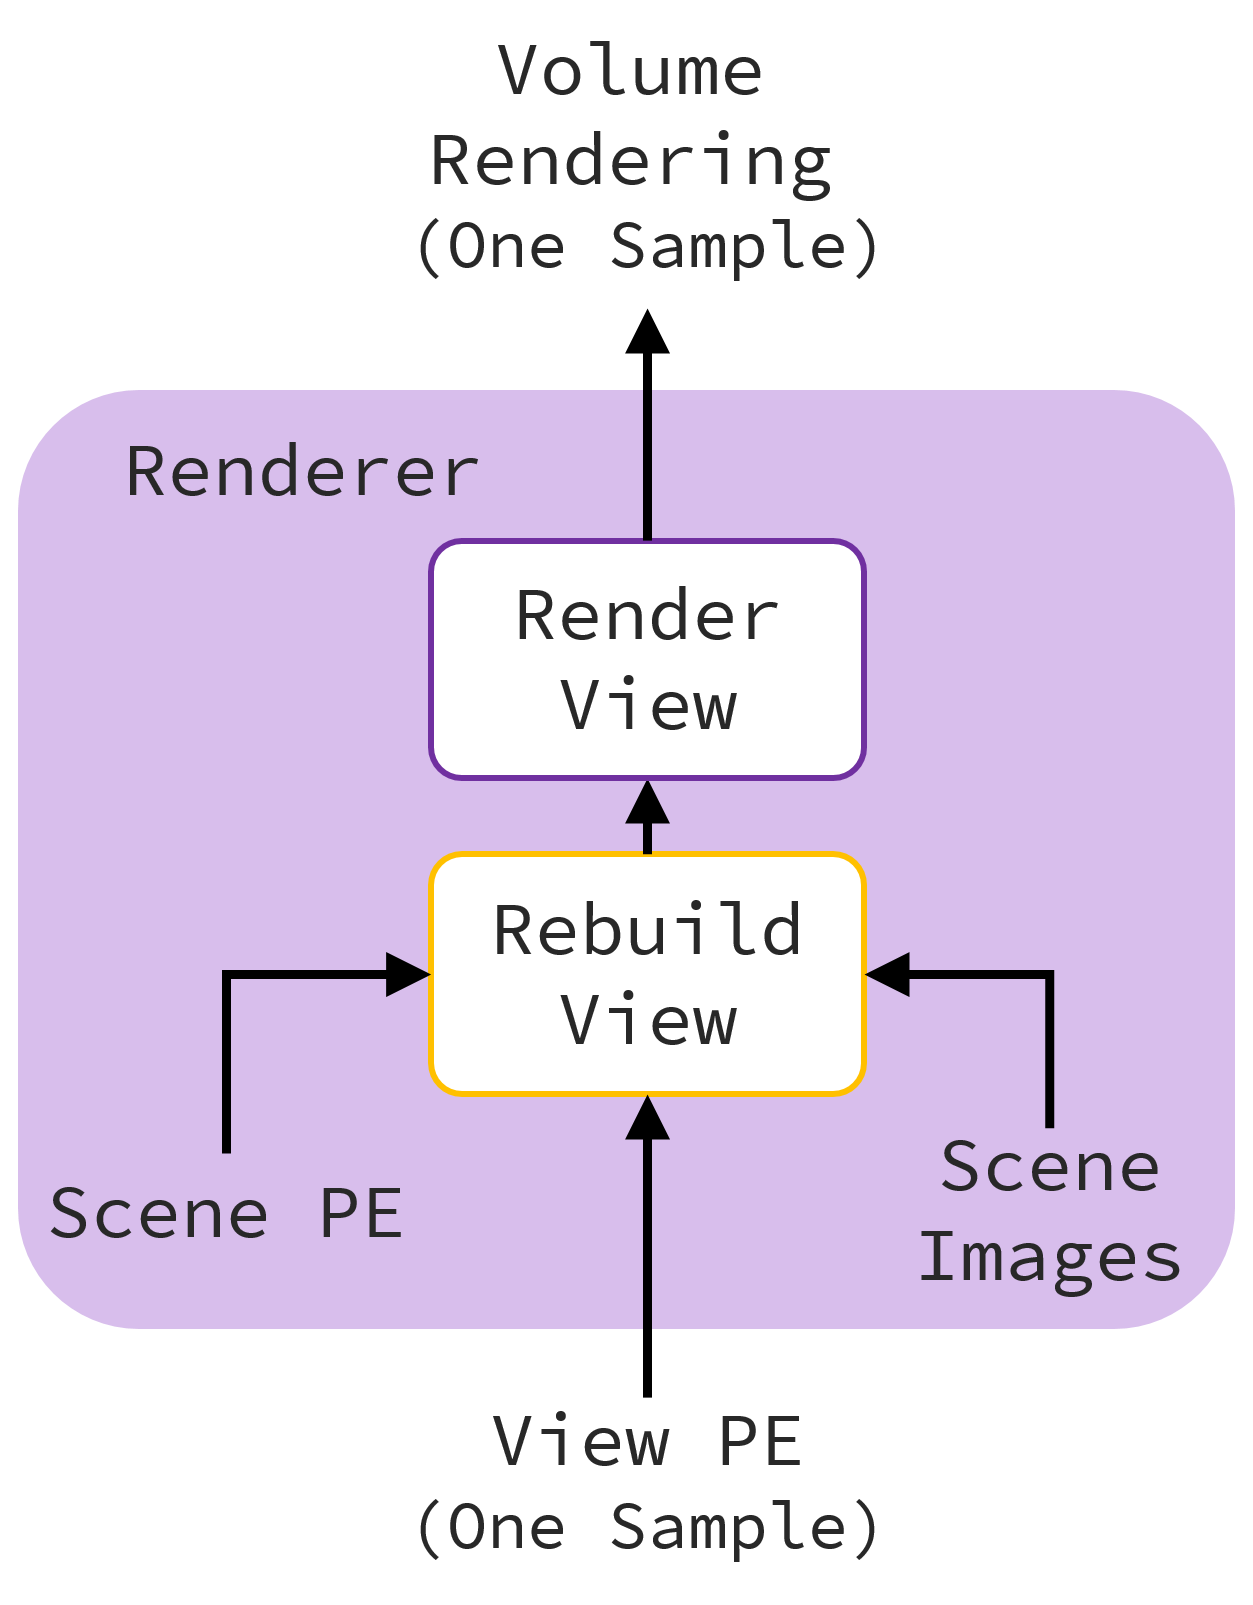
\includegraphics[width=0.8\linewidth]{img/NeRF-is-content-coupling.png}
      \end{center}
      \caption{
         NeRF 的設計使 Scene 與 Renderer 具有高度耦合性,使 Scene 內嵌於模型當中無法分離。
      }
      \label{fig:NeRF-is-content-coupling}
   \end{figure}

   然而,在一般 3D 場景的儲存與展示都是將 Scene 及 Renderer 拆分開來,並將 Scene
   作為輸入以取得對應視角的照片。這樣一來,Renderer 的部分就能重複利用於不同的
   3D 場景上。對應於原本 NeRF 中,訓練所使用的照片便相當於嵌入在 NeRF
   內的場景,若可以將照片改用於模型的輸入,便可將 Scene 與 Renderer 解耦合。
   \begin{figure}[t]
      \begin{center}
         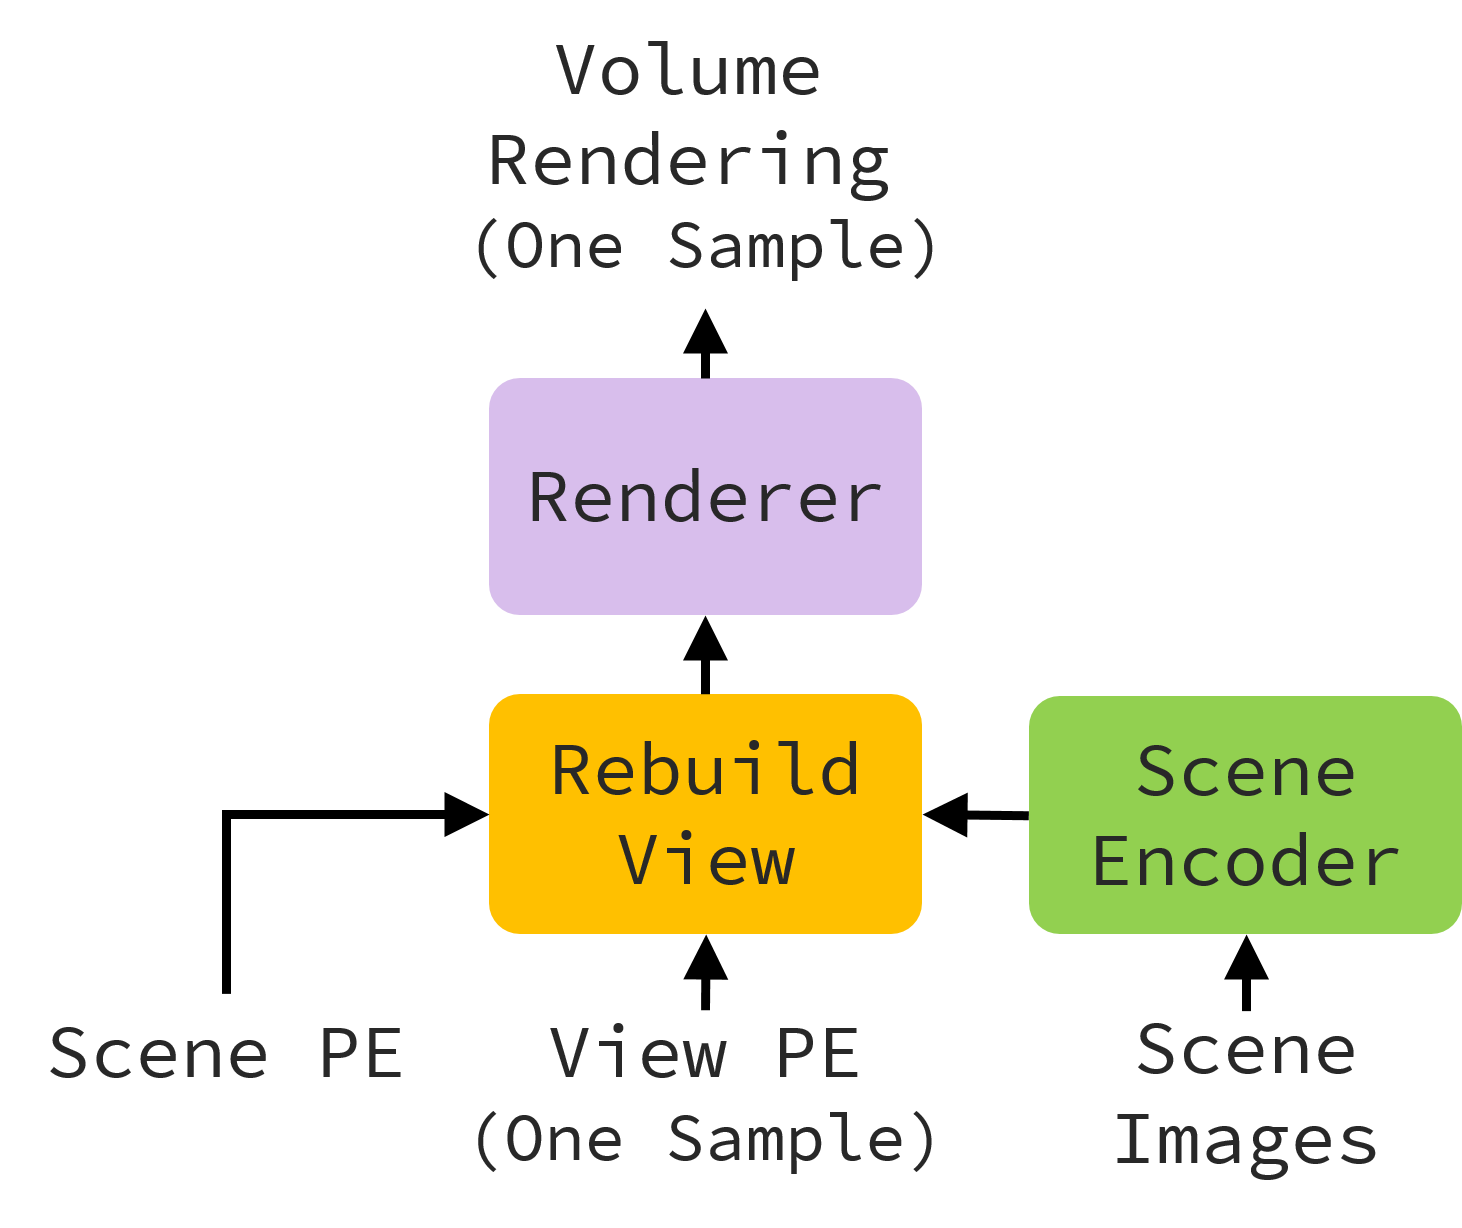
\includegraphics[width=0.9\linewidth]{img/Decoupling-NeRF.png}
      \end{center}
      \caption{
         本次專題所提出的 Decoupling-NeRF 就是希望將 Scene
         資訊與 Rebuild View 獨立出來。當要替換繪製場景時就不需要再經過耗時的訓練,只需要變更輸入的
         Scene Images 跟 Scene Position Encoding 即可。
      }
      \label{fig:Decoupling-NeRF}
   \end{figure}

   \begin{figure}[t]
      \begin{center}
         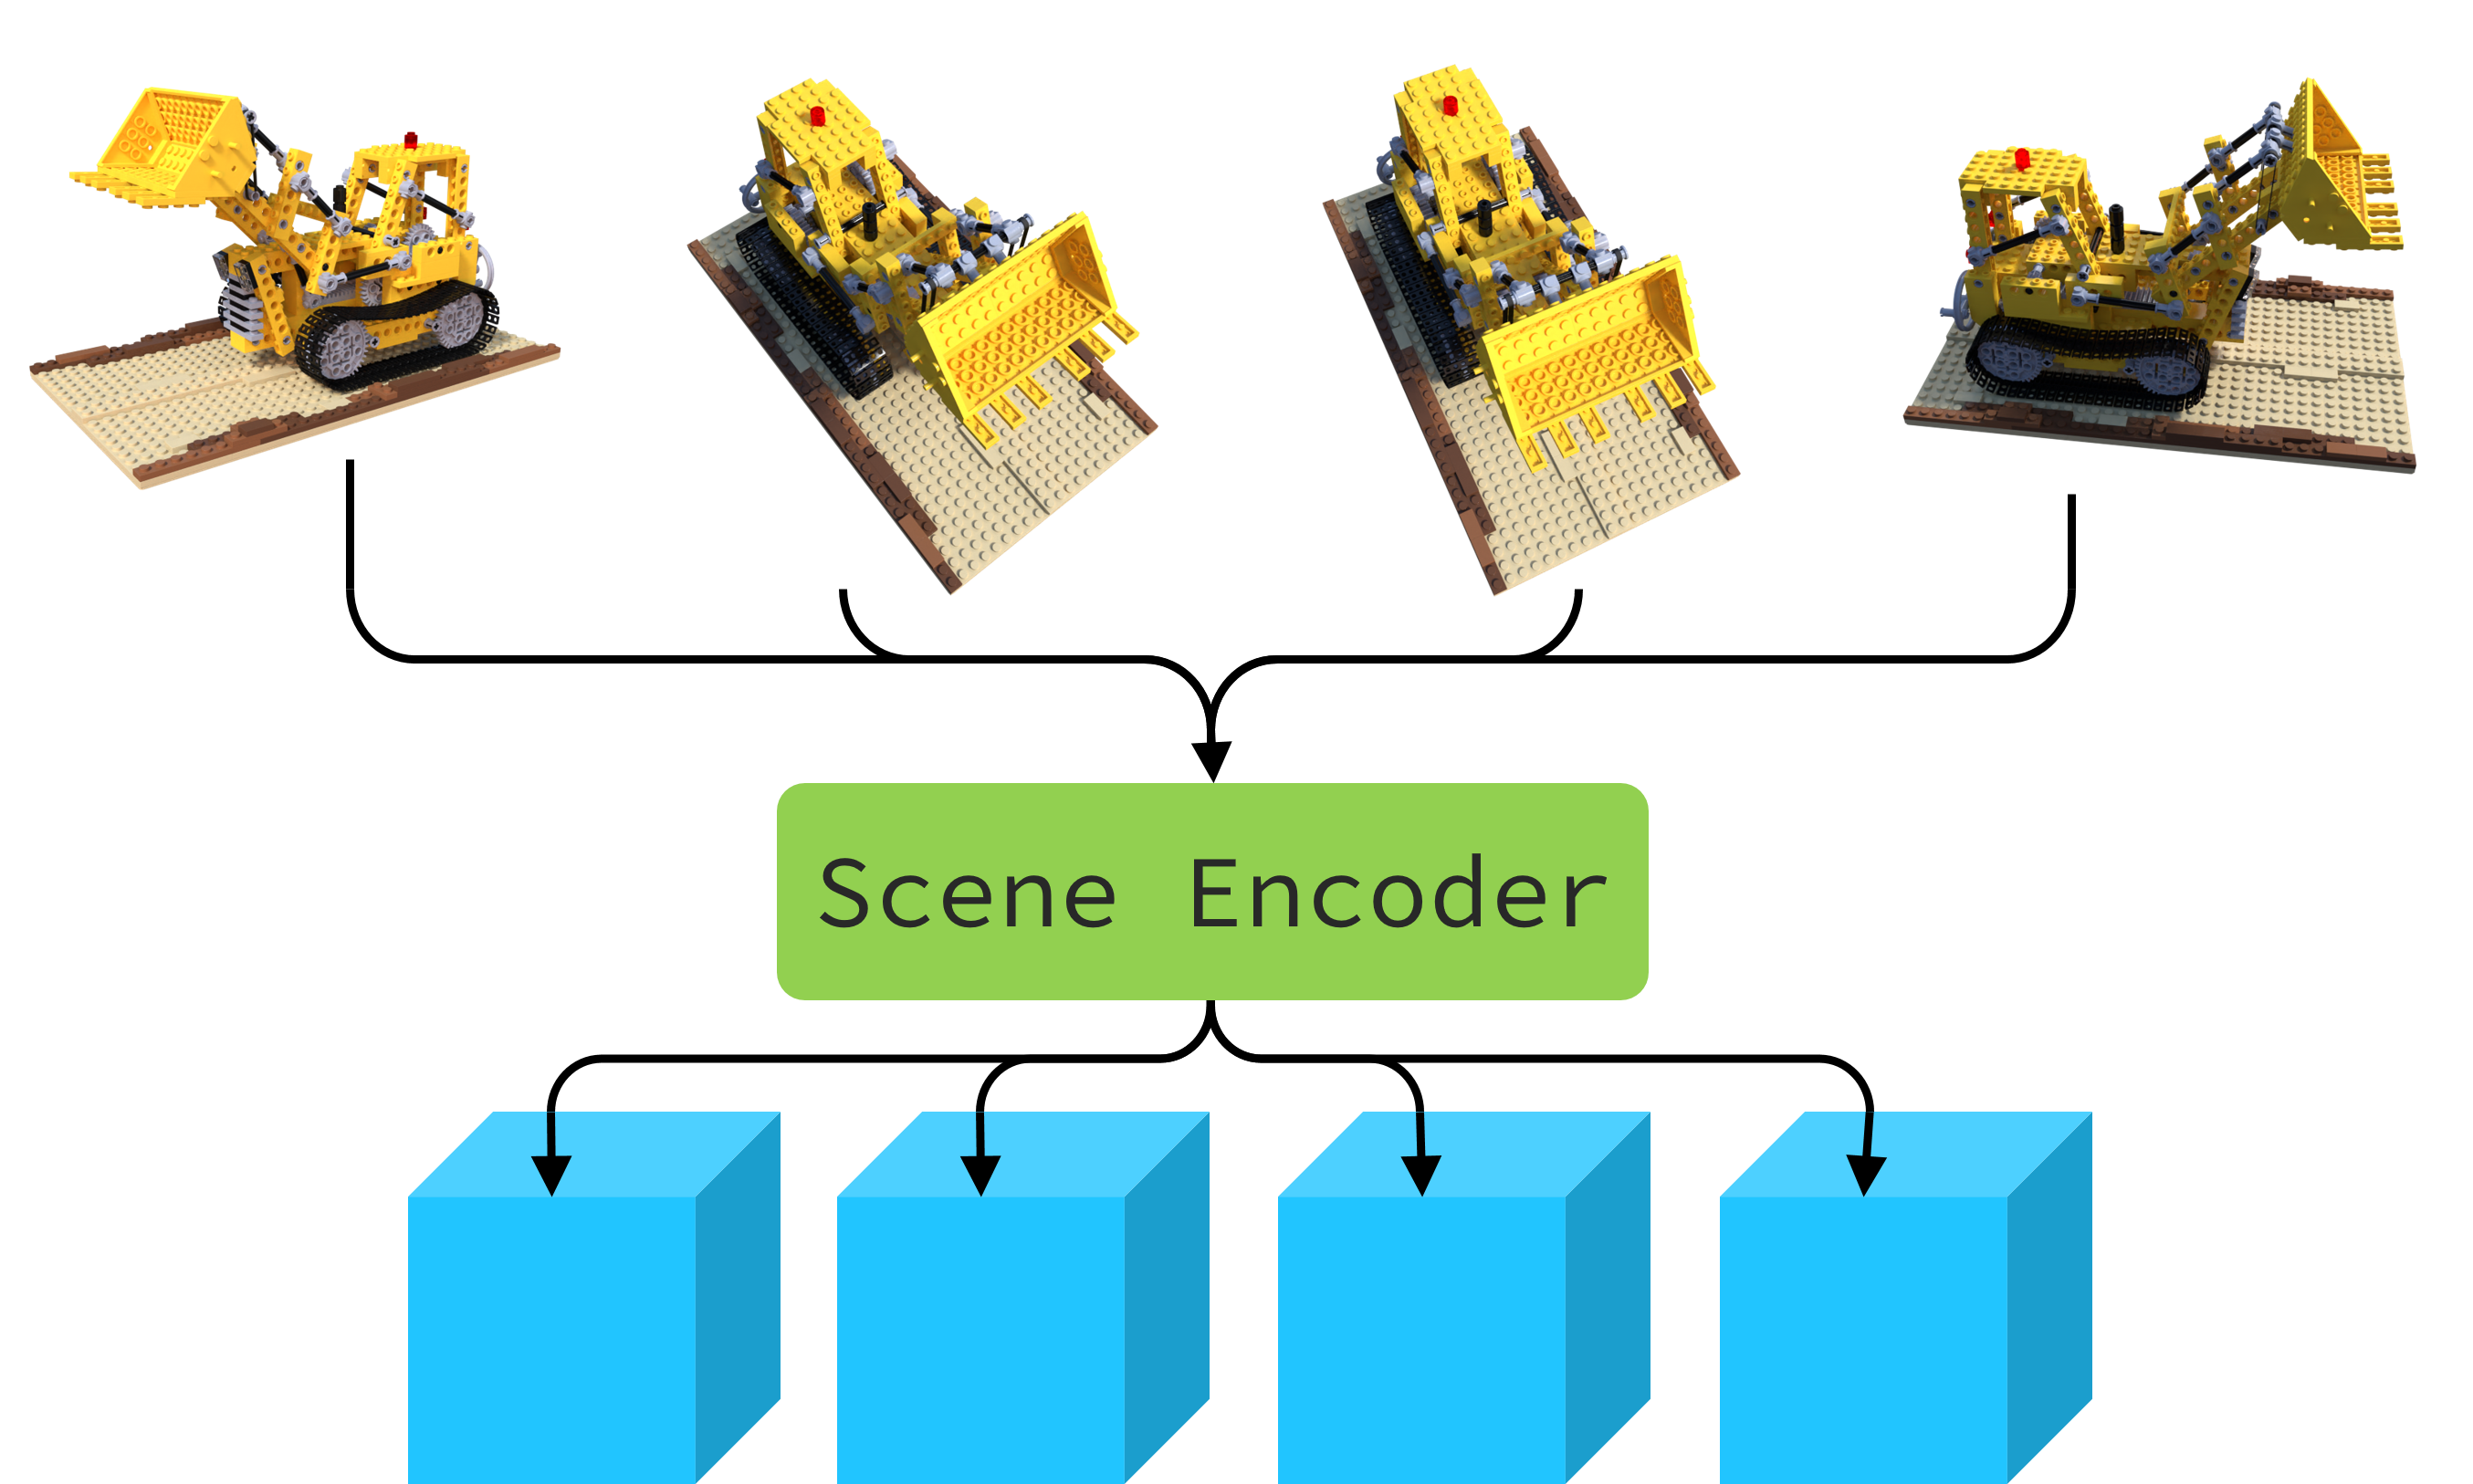
\includegraphics[width=1\linewidth]{img/encode-scene.png}
      \end{center}
      \caption{
         將場景照片透過 Encoder 編碼成 Scene Embedding。
      }
      \label{fig:encode-scene}
   \end{figure}

   \begin{figure*}
      \begin{center}
         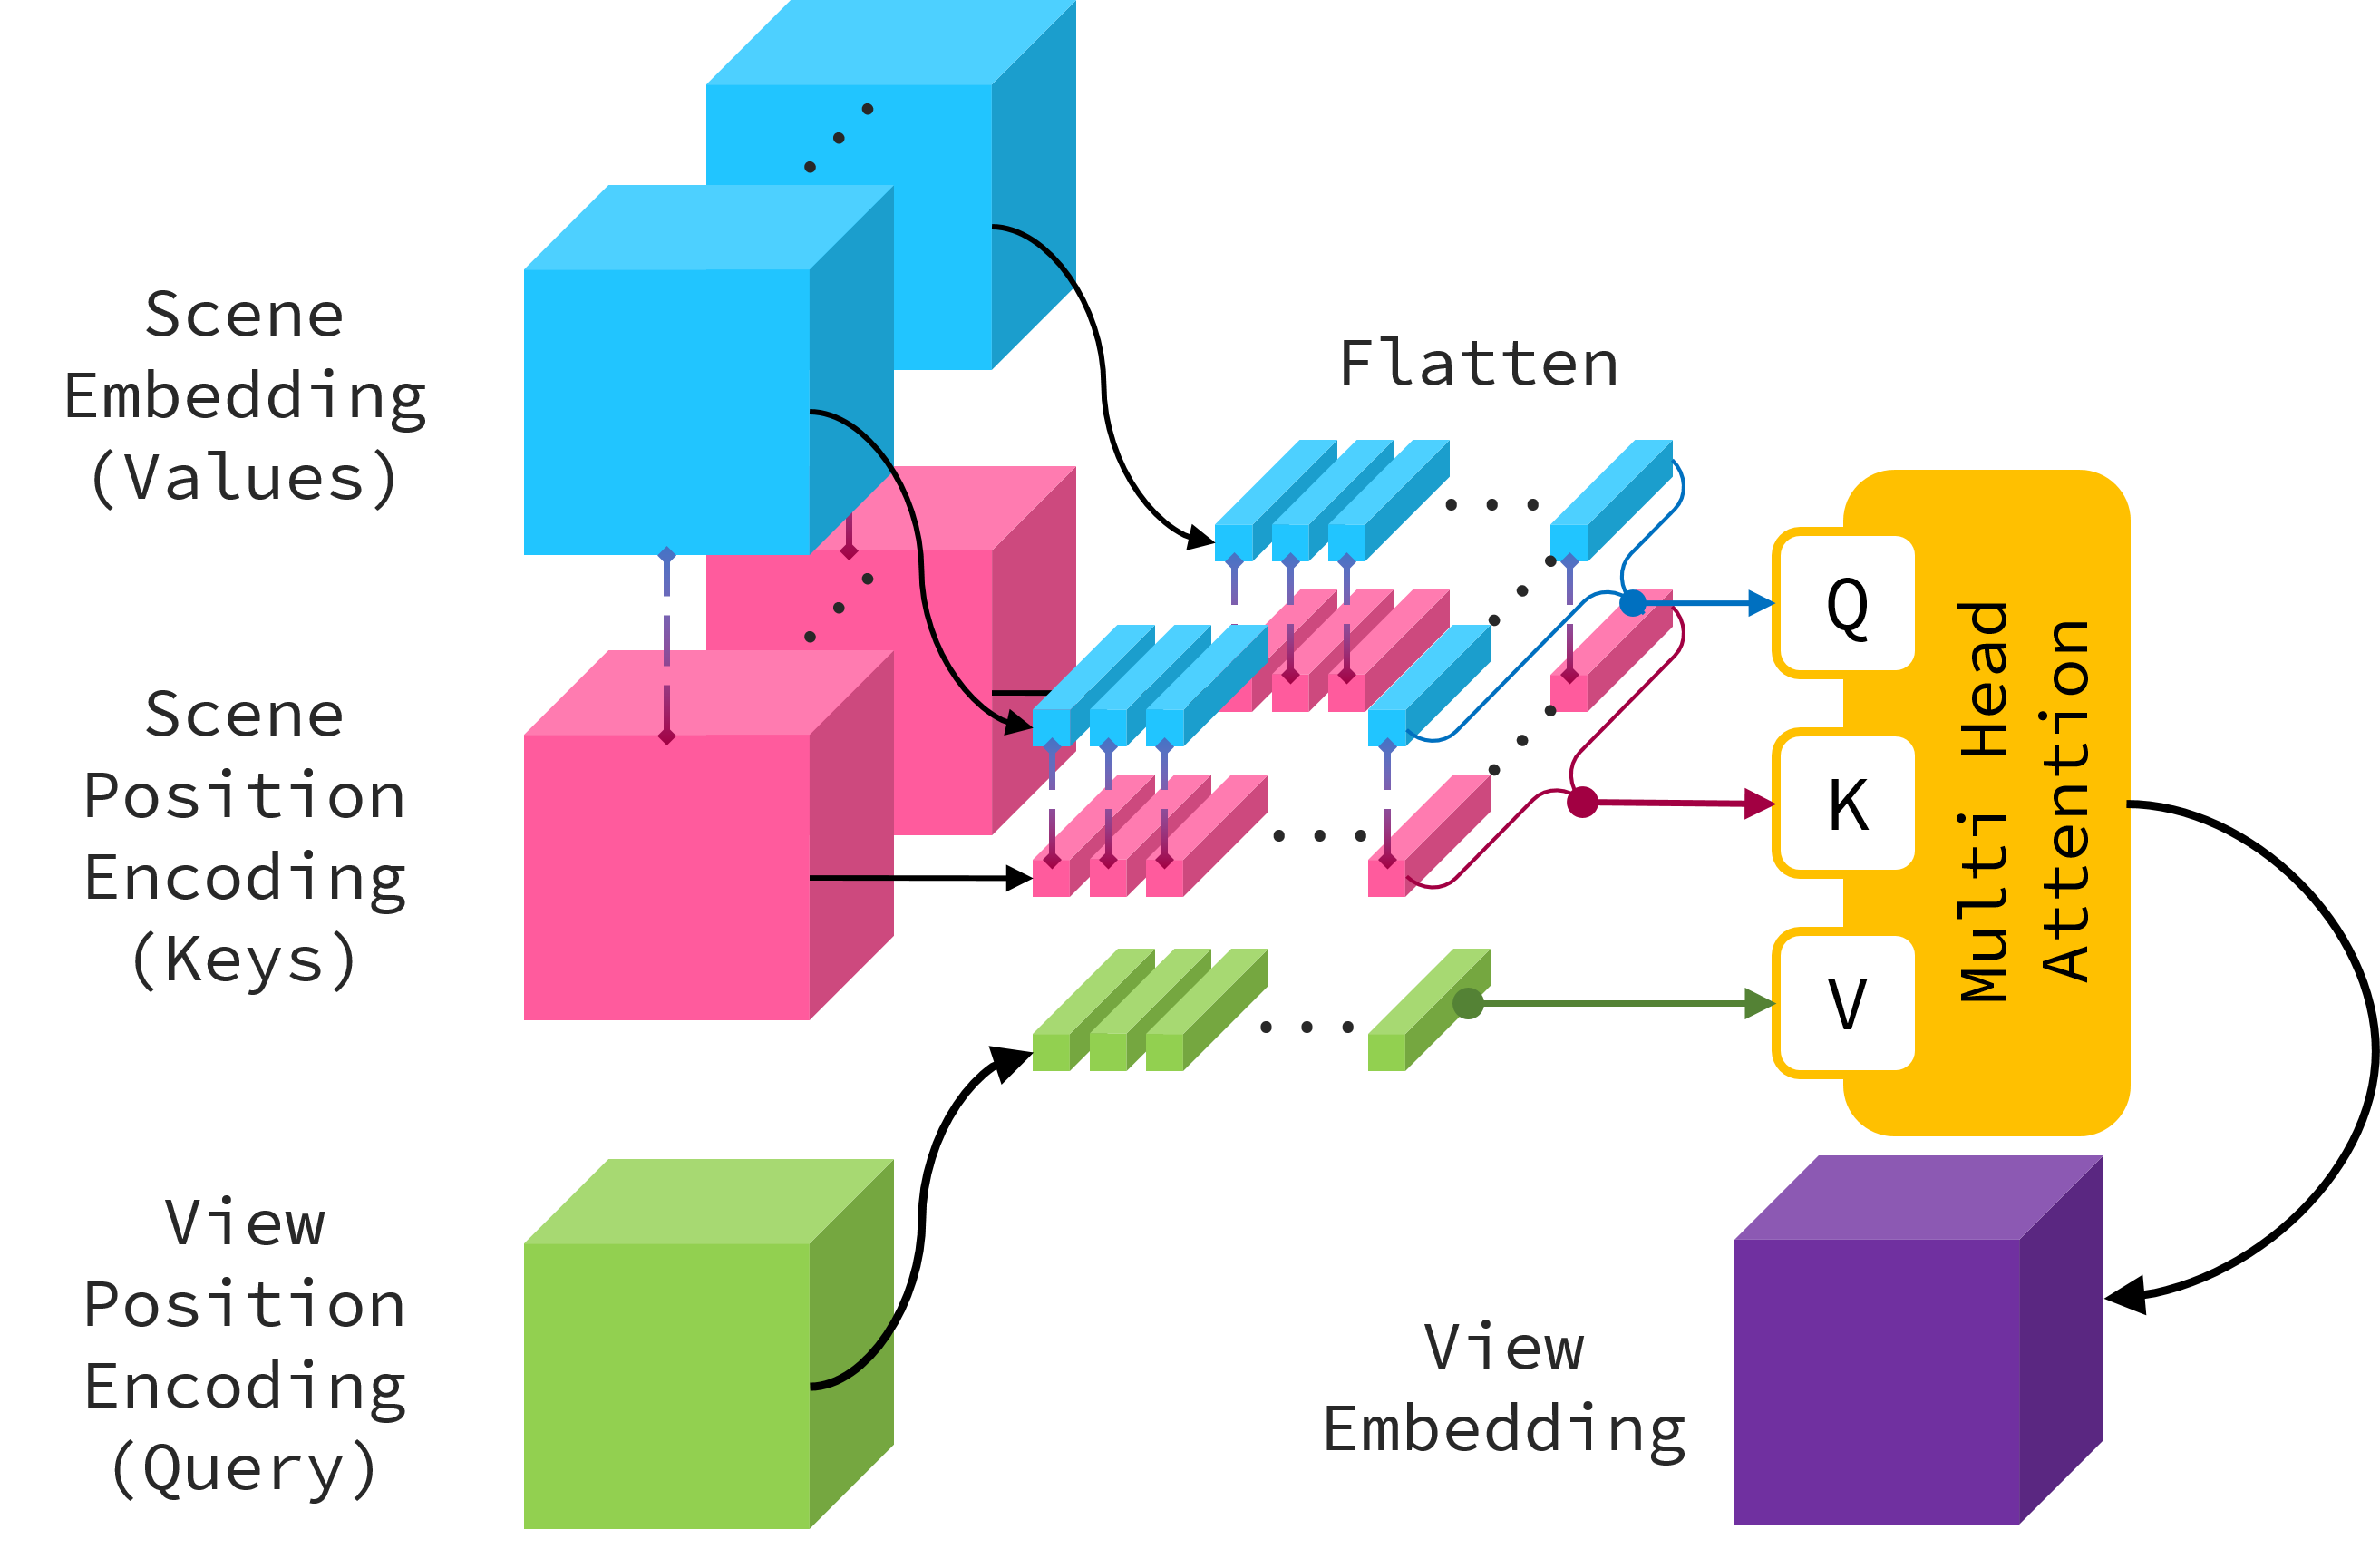
\includegraphics[width=1\linewidth]{img/rebuild-view.png}
      \end{center}
      \caption{
         將目標視角的位置編碼作為 Querys,與 Scene Embedding 及其對應的位置編碼計算
         Multi Head Attention 來取得 View Embedding。
      }
      \label{fig:rebuild-view}
   \end{figure*}

   因此,本次專題研究目標便是提出 Decoupling-NeRF 這個架構,使其可以快速應用在各種場景而不需要重新擬合。
   Fig.~\ref{fig:Decoupling-NeRF} 是本次專題的架構,將隱含於 NeRF
   中的 Renderer 與 Rebuild 分開,並利用 Scene Encoder
   對場景照片進行編碼,在 Rebuild View 使用 Multi Head Attention~\cite{AttentionIsAllYouNeed}
   將其重新組建為 View Embedding,最後透過單一 Neural Renderer 生成場景照片。

   \begin{figure}[htbp]
      \begin{center}
         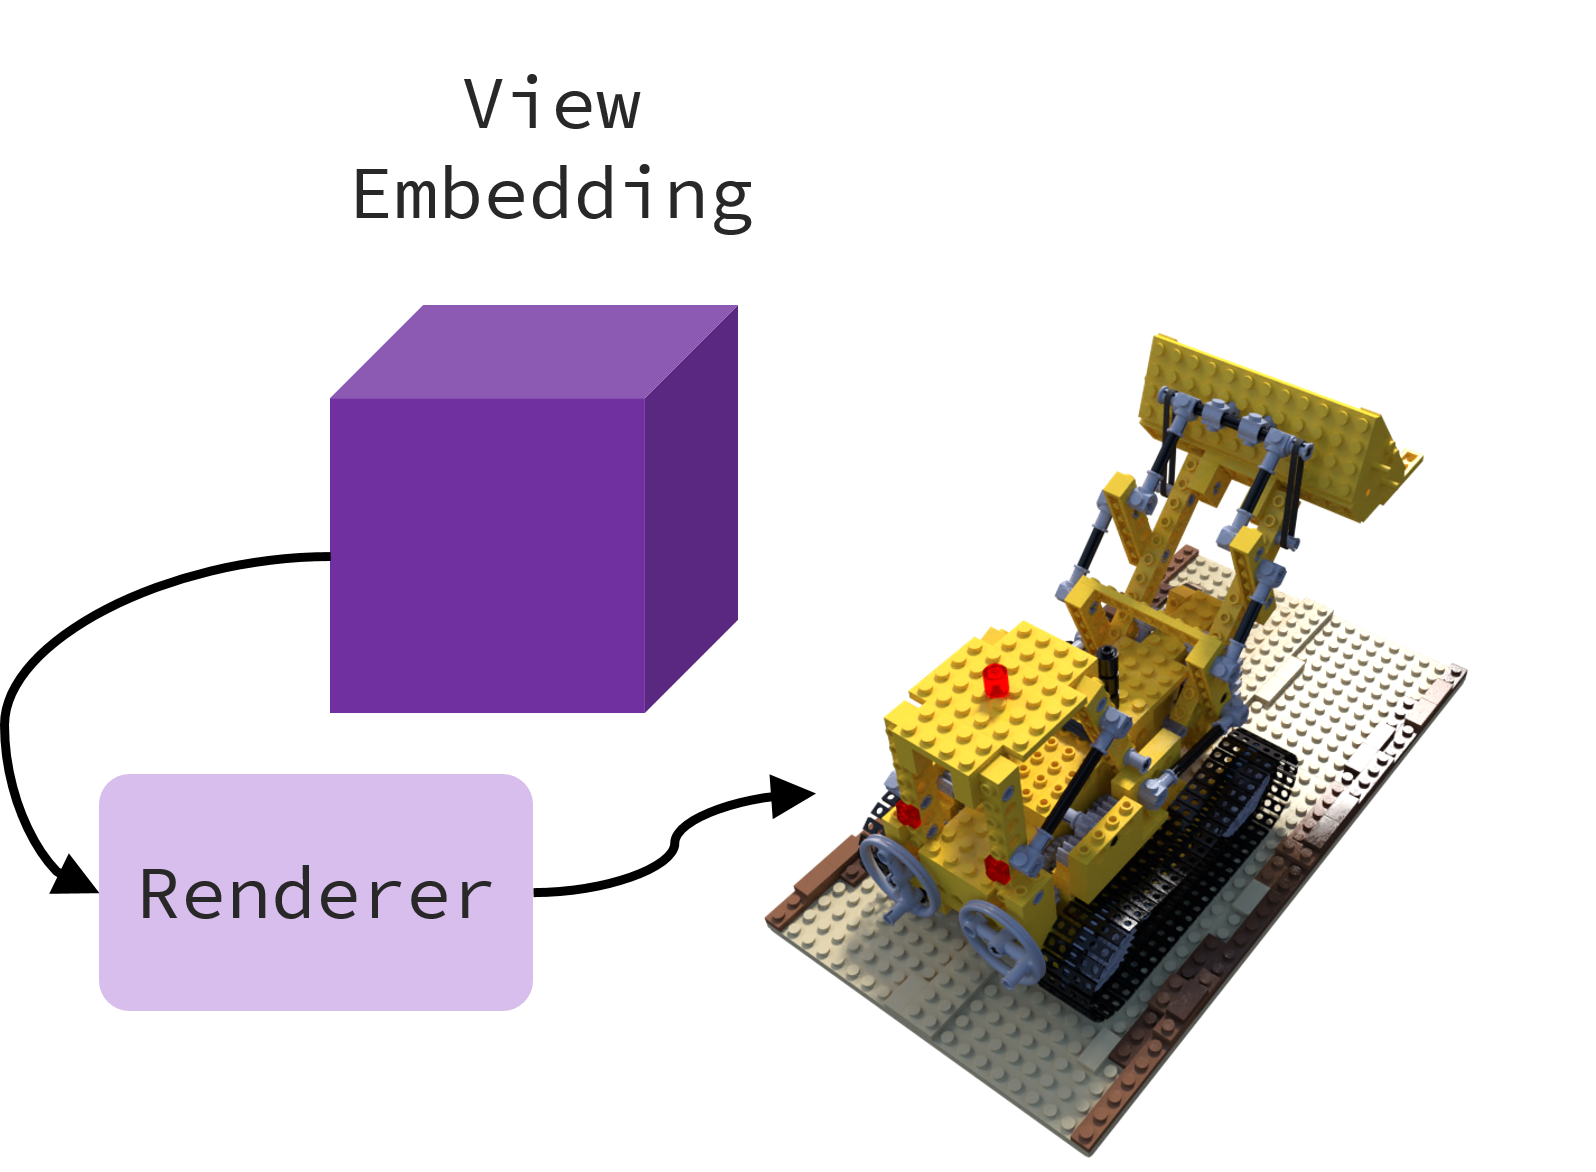
\includegraphics[width=1\linewidth]{img/render-view.png}
      \end{center}
      \caption{
         將 Fig.~\ref{fig:rebuild-view} 得到的 View Embedding 交由
         Renderer 進行 Volume Rendering。
      }
      \label{fig:render-view}
   \end{figure}

   \begin{figure}[htbp]
      \begin{center}
         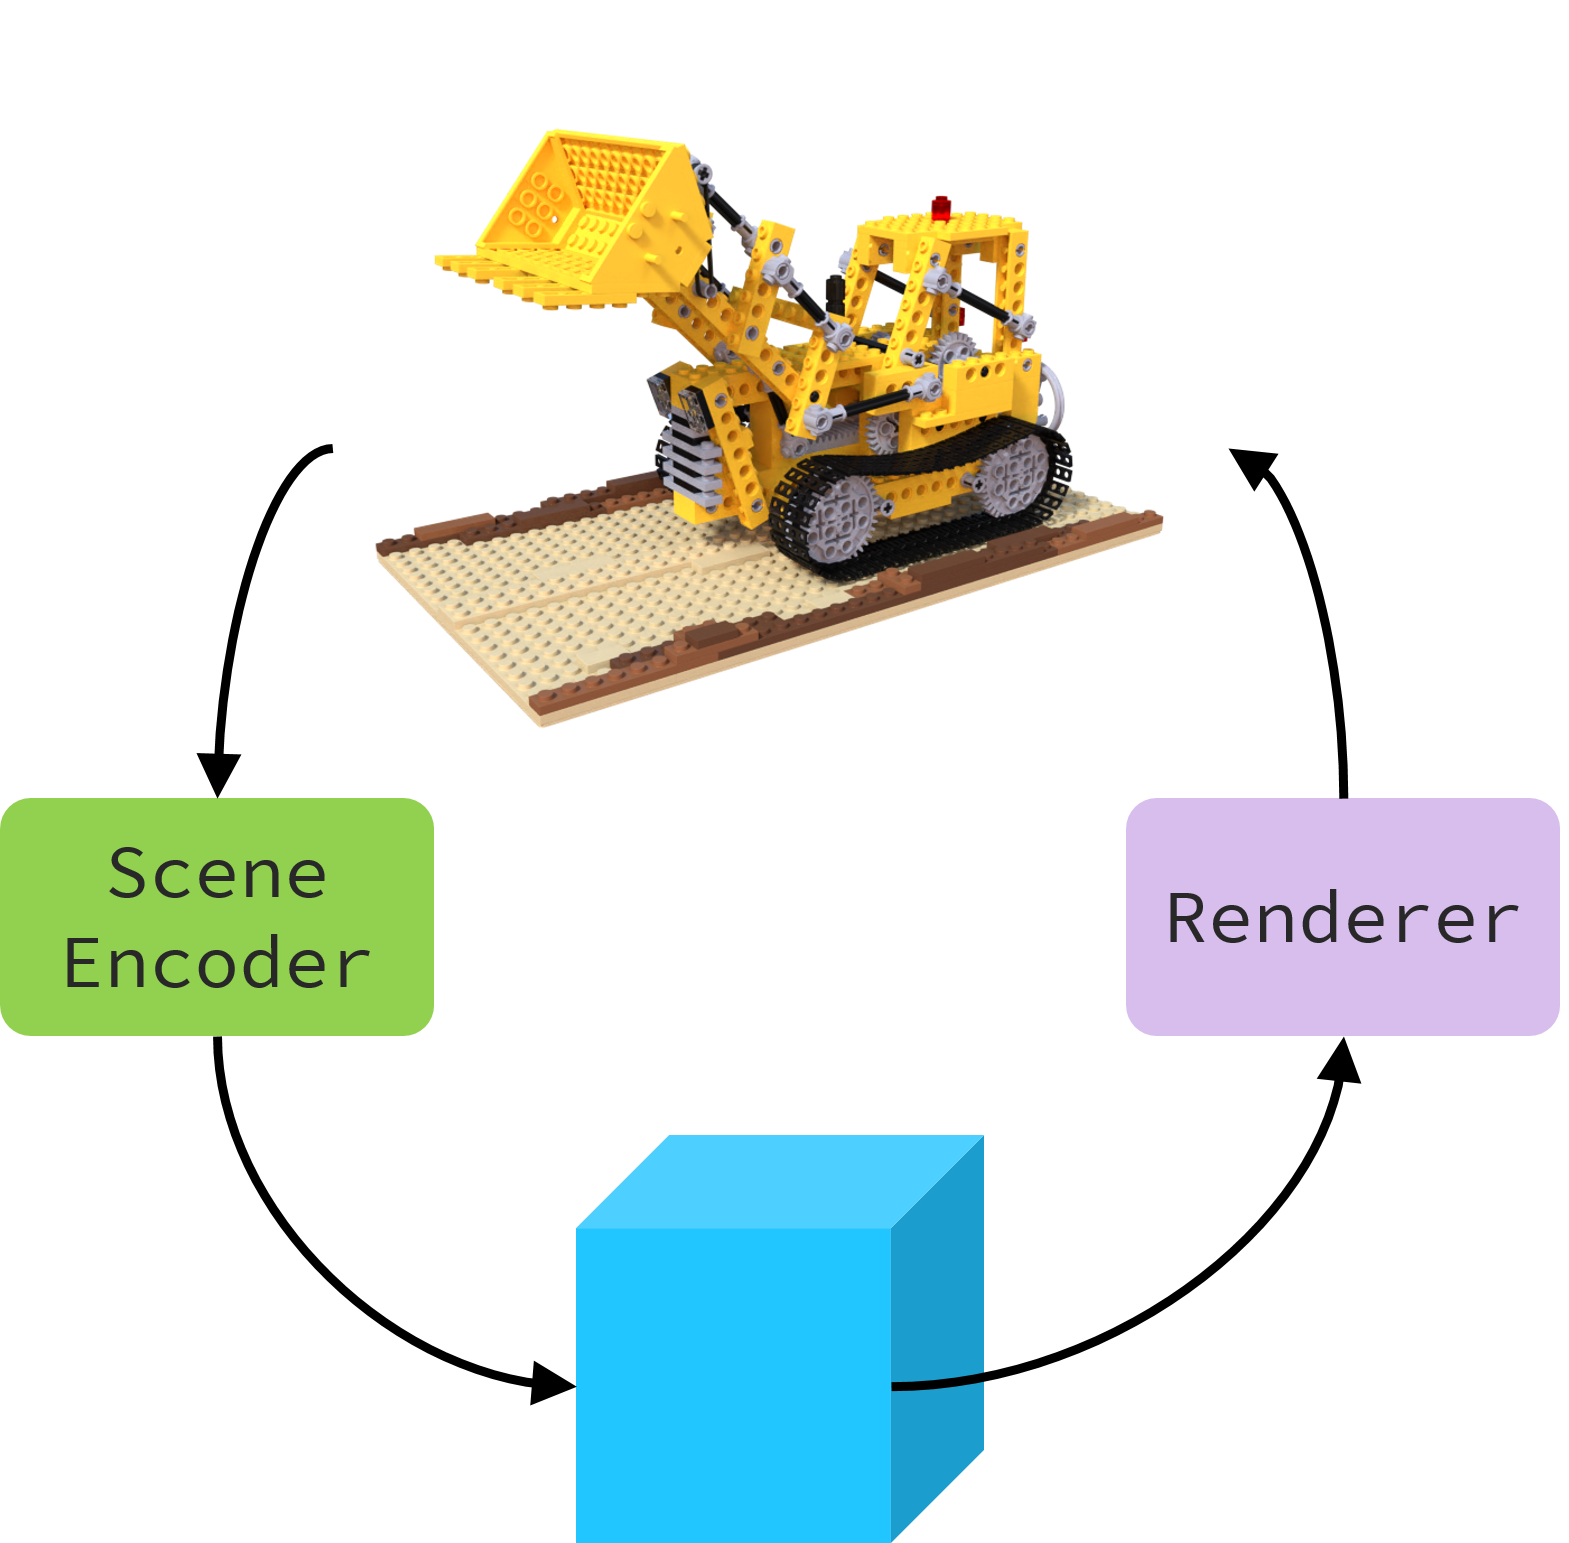
\includegraphics[width=1\linewidth]{img/auto-encoder.png}
      \end{center}
      \caption{
         預先訓練 Auto Encoder。
      }
      \label{fig:auto-encoder}
   \end{figure}
   %------------------------------------------------------------------------
   \section{System framework}

   在原版的 NeRF 中,會使用目標視角的位置編碼(Position Encoding,
   PE)作為輸入,以生成該視角會拍攝到場景照片,而 Position Encoding
   是將相機的位置資訊 Eq.~\ref{eq:position-encoding} 轉換所得:
   \begin{equation}
      \begin{aligned}
         PE(p)=[sin(2^{0}{\pi}{p}),~cos(2^{0}{\pi}{p}),~..., \\
         sin(2^{L-1}{\pi}{p}),~cos(2^{L-1}{\pi}{p})]
      \end{aligned}
      \label{eq:position-encoding}
   \end{equation}

   本專題架構如 Fig.~\ref{fig:Decoupling-NeRF} 所示,可以分成 Scene Encoder、Rebuild View 與 Renderer
   三個區塊。在進行照片生成時,先將多張場景照片編碼成 Scene Embedding(Fig.~\ref{fig:encode-scene}),再配合對應的 Scene PE 及生成目標的 View
   PE,將這三者以 Fig.~\ref{fig:rebuild-view} 的形式建立出
   View Embedding,最後再交由 Renderer 產生視圖(Fig.~\ref{fig:render-view})。

   在 Fig.~\ref{fig:rebuild-view} 中,利用了 Vaswani et al.~\cite{AttentionIsAllYouNeed} 所提出的
   Multi Head Attention 來將 Scene Embedding 重新組織成需要的 View Embedding。其計算方法如 Eq.~\ref{eq:multi-head-attention}:
   \begin{equation}
      \begin{aligned}
         MHA(Q, K, V) = Concat(head_{1},...,head_{h})W^{O}      \\
         head_{i} = Attention(QW^{Q}_{i},KW^{K}_{i},VW^{V}_{i}) \\
         Attention(Q, K, V ) = softmax(\frac{QK^{T}}{\sqrt{d_{k}}})V
      \end{aligned}
      \label{eq:multi-head-attention}
   \end{equation}

   在訓練階段則可分為兩個步驟,第一步會把架構中的 Scene Encoder 及 Renderer 以 Auto Encoder 的形式進行預訓練(如
   Fig.~\ref{fig:auto-encoder})。而步驟二不僅要訓練 Rebuild View,還會讓 Renderer 再次學習。

   %------------------------------------------------------------------------
   \section{Expected results}
   本專題將會使用 NeRF 提供的資料集\footnote{Link https://drive.google.com/drive/folders/128yBriW1IG\_3NJ5Rp7APSTZsJqdJdfc1}進行訓練與測試,其中提供了
   8 種場景與 8 個物件的多張照片及拍攝視角,並已區分成訓練、驗證跟測試集。

   在將模型訓練完成後,會測試不同數量的場景照片對模型生成能力所造成的影響。期望能將其製作成網頁應用,在計算能力有限的行動裝置下也能使用。

   {\small
   \bibliographystyle{ieee_fullname}
   \bibliography{egbib}
   }
\end{CJK}
\end{document}
